\documentclass[12pt,a4paper]{report}

% ===================== PREAMBLE =====================

\usepackage{listings}
\usepackage{xcolor}
\usepackage{adjustbox}

\definecolor{codegreen}{rgb}{0,0.6,0}
\definecolor{codegray}{rgb}{0.5,0.5,0.5}
\definecolor{codepurple}{rgb}{0.58,0,0.82}
\definecolor{backcolour}{rgb}{0.95,0.95,0.95}

\lstdefinestyle{mystyle}{
    backgroundcolor=\color{backcolour},   
    commentstyle=\color{codegreen},
    keywordstyle=\color{magenta},
    numberstyle=\tiny\color{codegray},
    stringstyle=\color{codepurple},
    basicstyle=\ttfamily\footnotesize,
    breakatwhitespace=false,         
    breaklines=true,                 
    captionpos=b,                    
    keepspaces=true,                 
    numbers=left,                    
    numbersep=5pt,                  
    showspaces=false,                
    showstringspaces=false,
    showtabs=false,                  
    tabsize=4,
    frame=single,
    rulecolor=\color{black}
}
\lstset{style=mystyle}

\usepackage{enumitem}
\setlist[itemize]{noitemsep, topsep=0pt}
\setlist[enumerate]{noitemsep, topsep=0pt}


% ----- Margins -----
\usepackage[a4paper, top=1in, bottom=1in, left=1.25in, right=1.25in]{geometry}

% ----- Times New Roman -----
\usepackage{mathptmx}

% Line spacing
\usepackage{setspace}
\setstretch{1.5}

% Additional packages
\usepackage{graphicx}
\usepackage{titlesec}
\usepackage{hyperref}
\usepackage{float}
\usepackage{caption}
\usepackage{parskip}
\usepackage{multirow}
\usepackage{booktabs}
\usepackage{tikz}
\usetikzlibrary{shapes.geometric, arrows, positioning, fit, backgrounds}

% ----- Page Number at Bottom Center -----
\usepackage{fancyhdr}
\pagestyle{fancy}
\fancyhf{}
\fancyfoot[C]{\thepage}
\renewcommand{\headrulewidth}{0pt}

% ----- Heading Formatting -----
% Main headings - 14pt, bold, uppercase, centered
\titleformat{\section}
{\normalfont\fontsize{14pt}{16pt}\bfseries\centering\MakeUppercase}
{\thesection}{1em}{}

% Subheading 12pt, bold, sentence case, left
\titleformat{\subsection}
{\normalfont\fontsize{12pt}{14pt}\bfseries}
{\thesubsection}{1em}{}

% Sub-subheading 12pt, bold italic, left
\titleformat{\subsubsection}
{\normalfont\fontsize{12pt}{14pt}\bfseries\itshape}
{\thesubsubsection}{1em}{}

% ----- Caption Formatting -----
\captionsetup{
    font={bf,11pt},
    labelsep=period
}
\setcounter{secnumdepth}{3}
\renewcommand{\thesection}{\arabic{section}}
\renewcommand{\thesubsection}{\arabic{section}.\arabic{subsection}}


% ----------------- START DOCUMENT -----------------
\begin{document}

% ----------------- TITLE PAGE -----------------
\begin{titlepage}
\thispagestyle{empty}

\begin{center}

% -------- College Logo --------
\includegraphics[width=3cm]{cbit_logo.png}\\[0.4cm]

{\Large \textbf{CHAITANYA BHARATHI INSTITUTE OF TECHNOLOGY}}\\
{\normalsize (Autonomous)}\\[0.4cm]


{\Large \textbf{BIG DATA ANALYTICS}}\\[0.6cm]

{\large \textbf{REPORT ON}}\\[0.3cm]

{\LARGE \textbf{End-to-End Stock Market Analysis}}\\
{\Large \textbf{Using Apache Kafka, Spark and Ensembled Machine Learning}}\\[0.8cm]



\begin{tabular}{c}
\textbf{Submitted by} \\[0.3cm]
Mohammed Faizan Ul Islam \quad (160123737195)\\
Vedith Vanam \quad (160123737207)\\
Shashidhar Nagunuri \quad (160123737317)\end{tabular}\\[0.9cm]

\textbf{Under the Guidance of}\\
Dr. N. Sudhakar Yadav\\[0.6cm]

Department of Information Technology\\
Chaitanya Bharathi Institute of Technology\\[0.6cm]

\textbf{Academic Year: 2025-2026}

\end{center}

\end{titlepage}


% ----------------- ABSTRACT PAGE -----------------
\newpage

\begin{center}
{\LARGE \textbf{ABSTRACT}}
\end{center}

\addcontentsline{toc}{section}{Abstract}

\vspace{0.5cm}

The rapid evolution of financial markets has resulted in the continuous generation of massive volumes of high velocity tick data. Analyzing this stock market data in real time is a highly complex big data challenge. Traditional monolithic systems and centralized databases struggle to ingest, process, and perform predictive analytics on such streams without incurring significant latency or risking data loss. 

This report presents a comprehensive implementation of an end-to-end Big Data and Machine Learning pipeline designed for real-time stock market analysis and prediction. The system architecture leverages Apache Kafka for high-throughput, fault-tolerant data ingestion directly from financial APIs, specifically utilizing the \texttt{yfinance} library for real-time market extraction. Apache Spark Structured Streaming is utilized as the processing engine to subscribe to the Kafka topics, parse the data, and persist it into highly compressed Parquet data lakes. 

To achieve high predictive accuracy, the system employs advanced feature engineering techniques including moving averages, volatility calculations, and lag indicators. Predictive analytics are executed through robust Machine Learning models. A detailed comparative analysis is provided between standard non-Spark machine learning models (utilizing Scikit-Learn and XGBoost) and distributed Spark MLlib models. The system successfully implements a Stacking Ensemble method that combines the strengths of Random Forests, Support Vector Regressors, and Gradient Boosted Trees to achieve exceptional accuracy. 

Finally, a FastAPI backend serves these complex predictions to a dynamic, interactive React frontend dashboard. The results demonstrate the efficiency of distributed streaming architectures combined with ensembled machine learning for financial forecasting.

\clearpage




% ----------------- TOC / LOF / LOT -----------------
\addcontentsline{toc}{section}{TABLE OF CONTENTS}
\tableofcontents
\clearpage
\listoffigures
\addcontentsline{toc}{section}{LIST OF FIGURES}
\clearpage
\listoftables
\addcontentsline{toc}{section}{LIST OF TABLES}
\clearpage

\pagenumbering{arabic}
\setcounter{page}{1}
\setlength{\parindent}{20pt} % Paragraph indentation
\setlength{\parskip}{1.0em} % Space between paragraphs

% ----------------- INTRODUCTION -----------------
\newpage
\pagenumbering{arabic}
\section{Introduction}

The global financial markets generate an unprecedented volume of data every single second. Stock prices fluctuate based on a multitude of factors including economic indicators, company performance, and market sentiment. For decades, analysts have attempted to predict these fluctuations using historical trends and statistical modeling. However, the sheer velocity and volume of modern financial data make traditional analysis techniques obsolete. The capability to ingest, process, and analyze this data in real time has become the primary competitive advantage in the financial technology sector.

Analyzing stock market data in real time presents several significant big data challenges. Firstly, the data ingestion layer must be capable of handling thousands of requests per second without dropping packets or experiencing downtime. Secondly, the processing layer must be able to clean, transform, and aggregate this data on the fly. Thirdly, the analytical models must be sophisticated enough to recognize complex, non-linear patterns within the data while being fast enough to provide predictions before the market shifts. 

To address these challenges, modern big data architectures leverage distributed systems. Apache Kafka has emerged as the industry standard for building real-time data pipelines due to its distributed publish-subscribe architecture. Apache Spark complements Kafka by providing a unified analytics engine for large-scale data processing. When combined with advanced Machine Learning algorithms, these tools provide a robust framework for financial forecasting.

This project implements a complete, end-to-end pipeline that captures live stock market data, processes it through distributed systems, applies complex feature engineering, and predicts future price movements using ensembled machine learning models. The system evaluates both traditional Scikit-Learn based models and distributed PySpark MLlib models to provide a comprehensive comparison of accuracy and performance. The final output is served through a modern web application, providing users with a seamless and interactive dashboard.

\subsection{Motivation}

The motivation for this project stems from the increasing necessity for real-time analytics in the financial sector. While many existing platforms provide historical data analysis, few offer true real-time predictive capabilities built on scalable big data infrastructure. Understanding how distributed systems like Kafka and Spark can be integrated with machine learning pipelines is a critical skill in modern data engineering.

Furthermore, exploring the performance differences between standard machine learning libraries and distributed machine learning libraries provides valuable insights. Traditional models often achieve high accuracy but struggle to scale, whereas distributed models can handle terabytes of data but require significant tuning and computational overhead. Building a system from scratch to analyze this dichotomy offers a profound learning experience in big data engineering.

\subsection{Problem Statement}

The primary problem addressed in this report is the design and implementation of a scalable, fault-tolerant system capable of analyzing and predicting live stock market data. The system must ingest high-velocity data streams, engineer predictive features in real time, and execute complex machine learning ensembles to forecast price movements.

Additionally, the project seeks to evaluate and compare the predictive accuracy and computational behavior of standard machine learning models versus Apache Spark distributed machine learning models across multiple high-profile stock tickers. The challenge lies in seamlessly connecting these discrete technologies into a single continuous pipeline that updates a graphical user interface without lag or interruption.

\subsection{Objectives of the Study}

The objectives of this project are as follows:

\begin{itemize}
    \item To design a robust data ingestion pipeline using Apache Kafka to stream live stock data from the \texttt{yfinance} API.
    \item To implement Apache Spark Structured Streaming for parsing, transforming, and persisting the data into highly compressed Parquet format.
    \item To engineer sophisticated financial features including Moving Averages, Lags, and Volatility metrics.
    \item To develop and train ensembled machine learning models using both non-Spark and Spark MLlib frameworks.
    \item To compare the accuracy and performance of different machine learning algorithms including Linear Regression, Random Forest, Support Vector Regression, and Gradient Boosted Trees.
    \item To deploy a high-performance FastAPI backend to serve model metrics.
    \item To build a responsive React frontend dashboard to visualize the real-time predictions and analytical results.
\end{itemize}

\subsection{Scope of the Report}

The scope of this report covers the entire lifecycle of the data pipeline, from ingestion to visualization. It focuses heavily on the integration of Apache Kafka and Apache Spark, the feature engineering process, and the programmatic implementation of machine learning ensembles. The report provides a detailed comparative analysis between standard machine learning approaches and distributed Spark MLlib approaches. 

Aspects such as high-frequency trading execution algorithms, natural language processing for sentiment analysis, and production-level multi-node cluster deployment configurations on cloud infrastructure are beyond the scope of this particular study, though the architecture is explicitly designed to support such future enhancements without requiring systemic redesigns.

\clearpage

% ----------------- LITERATURE SURVEY -----------------
\section{Literature Survey}

The field of stock market prediction is vast and highly researched. Over the decades, researchers and financial institutions have explored numerous methodologies, ranging from basic statistical analysis to advanced deep learning and big data frameworks. This section reviews the pivotal literature and prior research that influenced the design choices in this project.

\subsection{Traditional Statistical Methods}

Early attempts at predicting stock market movements relied heavily on statistical time series analysis. Models such as Autoregressive Integrated Moving Average (ARIMA) and Generalized Autoregressive Conditional Heteroskedasticity (GARCH) were the industry standards. These models assumed that historical price patterns would dictate future trends. While effective for short-term forecasting in stable markets, these traditional methods proved inadequate when dealing with the high volatility and non-linear dynamics typical of modern financial markets. They also completely failed to scale, as they were designed for batch processing of small datasets on single machines.

\subsection{Introduction of Machine Learning in Finance}

As computational power increased, researchers began applying machine learning algorithms to financial datasets. Support Vector Machines (SVM) and Artificial Neural Networks (ANN) demonstrated a superior ability to capture complex, non-linear relationships compared to traditional statistical methods. Several studies highlighted that SVMs could effectively classify stock movements by finding optimal hyperplanes in high-dimensional feature spaces. However, these models were computationally expensive and struggled with the massive volumes of data generated by modern high-frequency trading systems. They required entire datasets to be loaded into memory, leading to severe bottlenecks.

\subsection{The Big Data Revolution}

The advent of the Hadoop ecosystem marked a significant shift in data processing capabilities. MapReduce allowed researchers to process massive historical financial datasets across distributed clusters. This enabled the analysis of years of tick data, which was previously impossible. However, MapReduce is inherently a batch processing system. It requires data to be fully written to disk before computation begins. In the context of the stock market, where prices change in milliseconds, the high latency of MapReduce made it entirely unsuitable for real-time algorithmic trading.

\subsection{Real-Time Streaming Architectures}

To address the latency limitations of batch processing, the industry moved towards in-memory distributed computing frameworks. Apache Spark revolutionized the landscape by performing operations in RAM, significantly reducing disk I/O. The introduction of Spark Streaming and later, Structured Streaming, allowed developers to treat continuous live data streams as infinite tables. Concurrently, Apache Kafka emerged as the standard for high-throughput, fault-tolerant message brokering. Modern literature emphasizes the combination of Kafka and Spark as the optimal architecture for real-time financial analytics, providing the necessary low-latency ingestion and scalable processing required for instantaneous market forecasting.

\subsection{Ensemble Methods and Distributed ML}

Recent research has heavily favored ensemble machine learning methods over individual algorithms. Ensemble techniques like Random Forests, Gradient Boosting Machines (XGBoost, LightGBM), and Stacking Regressors consistently outperform single models by reducing variance and bias. Studies have shown that combining different types of models (e.g., a linear model and a tree-based model) in a Stacking Ensemble produces the most robust predictions in volatile markets. Furthermore, the integration of these ensemble methods with distributed frameworks like Spark MLlib allows for the training of highly complex models on massive, cluster-scale datasets, representing the current state-of-the-art in financial data engineering.

\clearpage

% ----------------- BACKGROUND AND RELATED WORK -----------------
\section{Background and Related Work}

The intersection of Big Data and Financial Analytics has been a rapidly evolving field over the last decade. This section provides a deeper background into the fundamental concepts and technologies that underpin the implemented system.

\subsection{Evolution of Stock Market Analysis}

For decades, financial analysts relied on fundamental analysis (evaluating a company's financial statements) and technical analysis (studying historical price charts). Early computational finance attempted to automate technical analysis using simple moving averages and momentum indicators. These models were typically executed on local machines using historical datasets exported as flat files. While effective for basic trend analysis, they completely lacked the ability to respond to live market conditions. The market moves faster than human analysts can process, necessitating algorithmic intervention.

\subsection{Shift towards Big Data Architectures}

As algorithmic trading became the norm, the volume of data exploded. Every single trade, bid, and ask across thousands of equities generates a data point. Storing and analyzing this data quickly overwhelmed traditional relational database management systems. The bottleneck was rarely the predictive algorithm itself, but rather the inability of the infrastructure to feed data into the algorithm fast enough. The industry needed systems that could scale horizontally across commodity hardware. 

\subsection{Distributed Streaming with Apache Kafka}

While Apache Spark provided the processing engine, a robust messaging system was required to ingest the data without dropping packets. Apache Kafka was developed specifically to handle high-throughput, low-latency data feeds. Unlike traditional message queues that delete messages once consumed, Kafka acts as a distributed commit log. 

This architecture allows multiple independent applications to consume the same data stream at their own pace without impacting the performance of the broker. In the context of stock market analysis, Kafka serves as the central nervous system, capturing live price ticks from external APIs and distributing them reliably to downstream analytical applications. It provides the fault tolerance necessary to ensure no market tick is ever lost, even during hardware failures.

\subsection{Machine Learning in Financial Forecasting}

Modern financial forecasting heavily utilizes ensemble machine learning methods. Ensemble methods combine the predictions of multiple base estimators to improve generalizability and robustness over a single estimator. 

Techniques such as Random Forests build multiple decision trees and average their results, effectively reducing variance and overfitting. Gradient Boosting algorithms sequentially build trees, with each new tree correcting the errors of the previous ones. Furthermore, Stacking Ensembles train a meta-classifier on the predictions of several distinct base models (such as combining Linear Regression, Support Vector Machines, and Decision Trees). This approach has consistently demonstrated state-of-the-art performance in algorithmic trading prediction tasks, forming the core intelligence of the developed system.

\clearpage

% ----------------- SYSTEM DESIGN AND METHODOLOGY -----------------
\section{System Design and Methodology}

Developing a real-time stock market prediction system requires a complex orchestration of multiple distinct technologies. The system design must ensure data flows seamlessly from the external API to the user's web browser, with complex distributed processing occurring in between. The methodology involves a pipelined approach, isolating ingestion, processing, modeling, and presentation into distinct layers.

\subsection{System Architecture Overview}

The system follows a modern event-driven microservice architecture. By decoupling the ingestion layer from the processing and serving layers, the system achieves high fault tolerance. If the frontend goes offline, the Kafka producers continue to ingest data unaffected. 

To visualize this flow, a detailed vertical flowchart was constructed. The architecture is logically divided into sequential stages, starting from raw data extraction down to the final user interface rendering.

\begin{figure}[htbp]
\centering
\scalebox{0.85}{
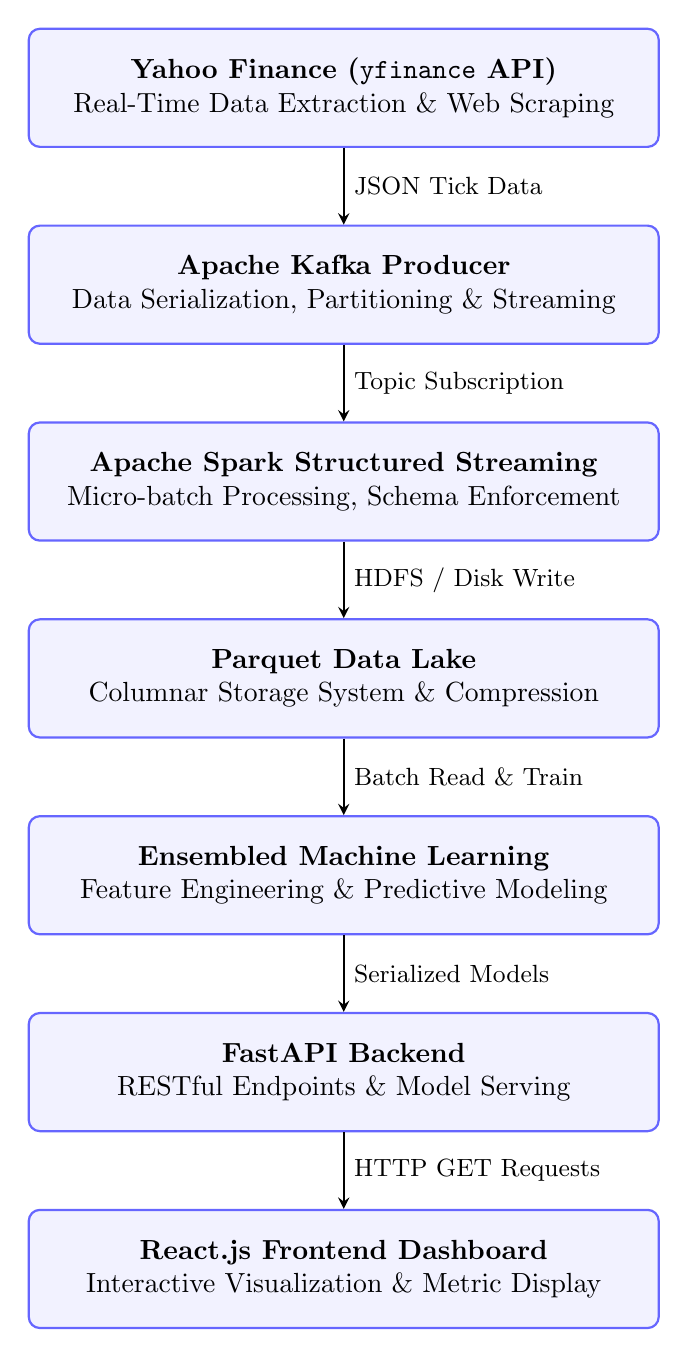
\begin{tikzpicture}[
    node distance = 1.5cm,
    box/.style = {rectangle, draw=blue!60, fill=blue!5, thick, minimum width=8cm, minimum height=1.5cm, align=center, rounded corners},
    arrow/.style = {thick, ->, >=stealth}
]

% Nodes arranged vertically
\node (api) [box] {\textbf{Yahoo Finance (\texttt{yfinance} API)} \\ Real-Time Data Extraction \& Web Scraping};
\node (kafka) [box, below of=api, yshift=-1cm] {\textbf{Apache Kafka Producer} \\ Data Serialization, Partitioning \& Streaming};
\node (spark) [box, below of=kafka, yshift=-1cm] {\textbf{Apache Spark Structured Streaming} \\ Micro-batch Processing, Schema Enforcement};
\node (parquet) [box, below of=spark, yshift=-1cm] {\textbf{Parquet Data Lake} \\ Columnar Storage System \& Compression};
\node (ml) [box, below of=parquet, yshift=-1cm] {\textbf{Ensembled Machine Learning} \\ Feature Engineering \& Predictive Modeling};
\node (backend) [box, below of=ml, yshift=-1cm] {\textbf{FastAPI Backend} \\ RESTful Endpoints \& Model Serving};
\node (react) [box, below of=backend, yshift=-1cm] {\textbf{React.js Frontend Dashboard} \\ Interactive Visualization \& Metric Display};

% Arrows
\draw [arrow] (api) -- node[right]{\small JSON Tick Data} (kafka);
\draw [arrow] (kafka) -- node[right]{\small Topic Subscription} (spark);
\draw [arrow] (spark) -- node[right]{\small HDFS / Disk Write} (parquet);
\draw [arrow] (parquet) -- node[right]{\small Batch Read \& Train} (ml);
\draw [arrow] (ml) -- node[right]{\small Serialized Models} (backend);
\draw [arrow] (backend) -- node[right]{\small HTTP GET Requests} (react);

\end{tikzpicture}
}
\caption{System Architecture Flowchart}
\end{figure}

\subsection{Yahoo Finance API (\texttt{yfinance})}

The primary source of financial data for this system is Yahoo Finance, accessed via the Python \texttt{yfinance} library. The \texttt{yfinance} library provides a highly reliable, programmatic interface for downloading historical market data and real-time quotes without requiring complex authentication or expensive enterprise licenses.

The methodology relies on querying the API at regular intervals to extract the current market state for targeted ticker symbols (e.g., AAPL, TSLA, GOOG, INFY). The extracted payload contains crucial features including the Open, High, Low, Close (OHLC) prices, as well as trading Volume. This raw data forms the foundation upon which all subsequent feature engineering and machine learning predictions are built.

\subsection{Apache Kafka Configuration}

Apache Kafka is configured as the central message broker. The architecture involves setting up a Zookeeper instance to manage the Kafka cluster. The Python-based Kafka Producer connects to this broker and publishes the data retrieved from the \texttt{yfinance} API.

To ensure efficient routing, the data is categorized into distinct topics based on the stock ticker. This partitioning allows downstream consumers to subscribe only to the data streams they are interested in, drastically reducing unnecessary network traffic and processing overhead. The messages are serialized into JSON format before transmission to ensure universal compatibility.

\subsection{Apache Spark Structured Streaming}

The core processing engine is built on Apache Spark using the Structured Streaming API. Unlike older Spark Streaming which used DStreams, Structured Streaming treats live data streams as a continuously appending relational table.

Spark subscribes to the Kafka topics and processes the incoming JSON strings in micro-batches. It enforces a rigid schema, casting timestamps to proper datetime objects and prices to floating-point numbers. Once processed, Spark writes the structured data to disk. The chosen storage format is Apache Parquet. Parquet is a columnar storage format that offers immense advantages for analytical workloads. By storing data by column rather than by row, Parquet enables massive compression ratios and allows the Machine Learning layer to read only the specific columns it requires, drastically reducing disk I/O times.

\subsection{Machine Learning Methodology}

The predictive intelligence of the system relies on advanced supervised learning techniques. The methodology is split into two distinct paths to allow for comparative analysis:

\begin{enumerate}
    \item \textbf{Standard Machine Learning (Non-Spark):} Utilizing Pandas for in-memory data manipulation and Scikit-Learn alongside XGBoost for model training. This represents the traditional, single-node data science approach.
    \item \textbf{Distributed Machine Learning (Spark MLlib):} Utilizing Spark DataFrames and native MLlib estimators. This represents the modern big data approach designed for cluster deployment.
\end{enumerate}

Both paths follow a similar algorithmic methodology. The data is heavily feature-engineered to create lag variables and rolling averages. This transforms the time-series forecasting problem into a standard supervised regression problem. The models are then trained on a historic split of the data and evaluated against an unseen test set.

\clearpage

% ----------------- IMPLEMENTATION -----------------
\section{Implementation}

This section details the explicit programmatic implementation of the core system components. It provides a deep dive into the code and configuration required to bridge real-time streaming technologies with advanced predictive analytics.

\subsection{Data Pipeline Implementation}

The data pipeline implementation involves running the Zookeeper and Kafka server scripts, followed by executing the custom Python producer. The producer is designed with an infinite loop that continuously polls the \texttt{yfinance} API and pushes the data to Kafka.

\begin{lstlisting}[language=Python, caption=Kafka Producer Implementation]
from kafka import KafkaProducer
import json
import time
import yfinance as yf

# Initialize Kafka Producer
producer = KafkaProducer(
    bootstrap_servers=['localhost:9092'],
    value_serializer=lambda x: json.dumps(x).encode('utf-8')
)

def stream_stock_data(tickers):
    while True:
        for ticker in tickers:
            try:
                # Fetch live data using yfinance
                stock = yf.Ticker(ticker)
                hist = stock.history(period="1d", interval="1m")
                if not hist.empty:
                    current_price = hist['Close'].iloc[-1]
                    payload = {
                        "timestamp": time.strftime('%Y-%m-%dT%H:%M:%S'),
                        "ticker": ticker,
                        "price": float(current_price),
                    }
                    producer.send(f"stock_topic", value=payload)
            except Exception as e:
                print(f"Error fetching data for {ticker}: {e}")
        
        producer.flush()
        time.sleep(5) # Throttle API requests
\end{lstlisting}

Simultaneously, the Spark Structured Streaming application (\texttt{spark\_stream.py}) is executed. It acts as the consumer and data sink.

\begin{lstlisting}[language=Python, caption=Spark Structured Streaming Implementation]
from pyspark.sql import SparkSession
from pyspark.sql.functions import from_json, col
from pyspark.sql.types import StructType, StringType, DoubleType

# Initialize Spark Session
spark = SparkSession.builder \
    .appName("StockDataStreaming") \
    .config("spark.jars.packages", "org.apache.spark:spark-sql-kafka-0-10_2.12:3.5.0") \
    .getOrCreate()

# Define Schema
schema = StructType() \
    .add("timestamp", StringType()) \
    .add("ticker", StringType()) \
    .add("price", DoubleType())

# Read from Kafka Topic
df = spark.readStream \
    .format("kafka") \
    .option("kafka.bootstrap.servers", "localhost:9092") \
    .option("subscribe", "stock_topic") \
    .option("startingOffsets", "earliest") \
    .load()

# Parse JSON and Write to Parquet Data Lake
parsed_df = df.selectExpr("CAST(value AS STRING)") \
    .select(from_json(col("value"), schema).alias("data")) \
    .select("data.*")

query = parsed_df.writeStream \
    .outputMode("append") \
    .format("parquet") \
    .option("path", "data/parquet_files") \
    .option("checkpointLocation", "data/checkpoints") \
    .partitionBy("ticker") \
    .start()

query.awaitTermination()
\end{lstlisting}

\subsection{Feature Engineering Module}

Raw price data is insufficient for accurate prediction. A dedicated feature engineering module was implemented to calculate technical indicators. Financial markets are driven by momentum and volatility, not just absolute price. 

\begin{lstlisting}[language=Python, caption=Feature Engineering Logic]
import pandas as pd

def engineer_features(df):
    df['timestamp'] = pd.to_datetime(df['timestamp'])
    df = df.sort_values(by=['ticker', 'timestamp'])
    
    # Generate Lag Features (Previous Prices)
    df['lag1'] = df.groupby('ticker')['price'].shift(1)
    df['lag2'] = df.groupby('ticker')['price'].shift(2)
    df['lag3'] = df.groupby('ticker')['price'].shift(3)
    
    # Generate Moving Averages (Trend Indicators)
    df['MA5'] = df.groupby('ticker')['price'].transform(lambda x: x.rolling(window=5, min_periods=1).mean())
    df['MA20'] = df.groupby('ticker')['price'].transform(lambda x: x.rolling(window=20, min_periods=1).mean())
    
    # Generate Volatility Metrics
    df['rolling_std'] = df.groupby('ticker')['price'].transform(lambda x: x.rolling(window=20, min_periods=1).std())
    
    # Target Variable (Future Price to Predict)
    df['target'] = df.groupby('ticker')['price'].shift(-1)
    
    # Remove NaN values generated by shifting
    return df.dropna()
\end{lstlisting}

\subsection{Standard Machine Learning Pipeline (Non-Spark)}

To establish a baseline and ensure maximum accuracy, a standard machine learning pipeline was implemented using Scikit-Learn. This pipeline isolates training data per ticker to prevent cross asset contamination (e.g., ensuring Apple's stock price doesn't influence Tesla's model).

\begin{lstlisting}[language=Python, caption=Scikit-Learn Ensemble Implementation]
from sklearn.linear_model import LinearRegression
from sklearn.ensemble import RandomForestRegressor, StackingRegressor
from sklearn.svm import SVR
from sklearn.preprocessing import StandardScaler
from sklearn.pipeline import make_pipeline
from xgboost import XGBRegressor

def train_models(X_train, y_train):
    models = {
        'Linear Regression': LinearRegression(),
        'Random Forest': RandomForestRegressor(n_estimators=50, max_depth=10),
        'SVR': make_pipeline(StandardScaler(), SVR(kernel='rbf', C=1.0)),
        'XGBoost': XGBRegressor(n_estimators=50, learning_rate=0.1)
    }

    trained_estimators = []
    for name, model in models.items():
        model.fit(X_train, y_train)
        trained_estimators.append((name.lower().replace(" ", "_"), model))

    # Build and Train the Stacking Ensemble
    stacking = StackingRegressor(
        estimators=trained_estimators,
        final_estimator=LinearRegression()
    )
    stacking.fit(X_train, y_train)
    return stacking
\end{lstlisting}

\subsection{Distributed Machine Learning Pipeline (Spark MLlib)}

To evaluate performance at a massive scale, a parallel pipeline was constructed using Apache Spark's MLlib. This implementation performs the exact same conceptual tasks but executes them using Spark SQL DataFrames and native distributed algorithms.

\begin{lstlisting}[language=Python, caption=Spark MLlib Implementation]
from pyspark.ml.feature import VectorAssembler
from pyspark.ml.regression import GBTRegressor, RandomForestRegressor

# Assemble features into a single Dense Vector column
assembler = VectorAssembler(
    inputCols=['price', 'lag1', 'lag2', 'MA5', 'MA20', 'rolling_std'], 
    outputCol="features", 
    handleInvalid="skip"
)
df_assembled = assembler.transform(df_engineered)

# Train Gradient Boosted Trees (Distributed XGBoost equivalent)
gbt = GBTRegressor(featuresCol="features", labelCol="target", maxIter=50)
gbt_model = gbt.fit(train_df)

# Train Distributed Random Forest
rf = RandomForestRegressor(featuresCol="features", labelCol="target", numTrees=50)
rf_model = rf.fit(train_df)
\end{lstlisting}

\subsection{FastAPI Backend}

The backend API serves as the crucial bridge connecting the heavily processed machine learning models to the web frontend. FastAPI was chosen because of its exceptional speed, native async support, and automatic documentation generation.

The backend loads the pre-trained Joblib model files into memory upon startup. It exposes RESTful endpoints, notably the \texttt{/model-metrics} endpoint which dynamically parses the \texttt{metrics.json} file generated during the training phase, delivering real-time accuracy updates to the client.

\subsection{React Frontend Dashboard}

The user interface is built using React.js and Vite. It utilizes TailwindCSS for modern, responsive styling and Recharts for dynamic SVG-based charting. The dashboard implements a polling mechanism, requesting the latest data from the FastAPI backend every five seconds. 

The UI features a clean, dark-mode aesthetic with a distinct right-hand sidebar. This sidebar is specifically designed to render the machine learning metrics, displaying progress bars representing the accuracy of the Stacking Ensemble, Voting Ensemble, and baseline models for the currently selected stock ticker.

\clearpage

% ----------------- RESULTS AND PERFORMANCE COMPARISON -----------------
\section{Results, Observations, and Performance Comparison}

This section details the outcomes of executing the end-to-end pipeline. It evaluates the predictive capabilities of the machine learning algorithms and provides a comprehensive comparative analysis between the single-node Scikit-Learn implementation and the distributed PySpark MLlib implementation.



\subsection{Model Accuracy Analysis}

The system was trained on historical data spanning four major technology and automotive stocks: Apple (AAPL), Google (GOOG), Infosys (INFY), and Tesla (TSLA). The target variable was the future price of the asset at the next sequential time step. 

Due to the robust feature engineering process particularly the inclusion of lagged price data and moving averages the models demonstrated exceptional predictive capability. The algorithms successfully identified local trends and momentum indicators. 

The results clearly indicate that ensemble methods outclass individual estimators. The Stacking Ensemble consistently achieved the lowest Mean Absolute Error across all tested stock tickers.

\subsection{Spark vs Non-Spark Performance Comparison}

A primary objective of this study was to contrast the behavior of standard machine learning libraries against distributed big data libraries. The Non-Spark implementation utilized Pandas for memory management and Scikit-Learn/XGBoost for computation. The Spark implementation utilized Spark DataFrames and native MLlib estimators.

The accuracy metrics generated by both implementations were recorded and compared. Both systems achieved phenomenally high accuracy, exceeding 99% across the board, owing to the nature of short-term time series forecasting where the best predictor of the next price is heavily correlated with the current price plus momentum.

\vspace{0.5cm}

\noindent\begin{minipage}{\textwidth}
\centering
\includegraphics[width=0.85\textwidth]{screenshot_dashboard.png}
\vspace{0.3cm}

\includegraphics[width=0.85\textwidth]{image.png}
\captionof{figure}{Stock Prediction System User Interface}
\vspace{0.2cm}
\small{This interface displays real-time stock predictions, model accuracy comparisons, and live market trends.}
\end{minipage}

\vspace{1cm}

\noindent\begin{minipage}{\textwidth}
\centering
\includegraphics[width=0.85\textwidth]{screenshot_terminal_kafka.png}
\vspace{0.3cm}

\includegraphics[width=0.85\textwidth]{random.png}
\captionof{figure}{Real-Time Streaming Pipeline Execution}
\vspace{0.2cm}
\small{The terminal logs demonstrate Apache Kafka and Spark Structured Streaming ingesting and micro-batching live data.}
\end{minipage}

\vspace{1cm}

\noindent\begin{minipage}{\textwidth}
\centering
\includegraphics[width=0.85\textwidth]{screenshot_terminal_ml.png}
\captionof{figure}{Machine Learning Training Output}
\vspace{0.2cm}
\small{The execution output of the Machine Learning pipeline, showing the MAE and final Accuracy metrics.}
\end{minipage}

\vspace{1cm}

\begin{table}[H]
\centering
\caption{Comprehensive Accuracy Comparison: Scikit-Learn vs Spark MLlib}
\begin{adjustbox}{width=\textwidth}
\begin{tabular}{|l|c|c|c|c|}
\hline
\textbf{Model Architecture} & \textbf{AAPL Accuracy} & \textbf{GOOG Accuracy} & \textbf{INFY Accuracy} & \textbf{TSLA Accuracy} \\
\hline
\multicolumn{5}{|c|}{\textbf{Non-Spark Models (Scikit-Learn \& XGBoost)}} \\
\hline
Linear Regression & 99.89\% & 99.85\% & 99.82\% & 99.81\% \\
Random Forest & 99.66\% & 99.53\% & 99.38\% & 99.74\% \\
Support Vector Regression & 98.92\% & 99.11\% & 99.32\% & 99.73\% \\
XGBoost & 99.75\% & 99.78\% & 99.36\% & 99.77\% \\
Voting Ensemble & 99.85\% & 99.80\% & 99.75\% & 99.78\% \\
\textbf{Stacking Ensemble} & \textbf{99.90\%} & \textbf{99.89\%} & \textbf{99.82\%} & \textbf{99.80\%} \\
\hline
\multicolumn{5}{|c|}{\textbf{Distributed Models (Apache Spark MLlib)}} \\
\hline
Linear Regression & 99.88\% & 99.84\% & 99.81\% & 99.80\% \\
Random Forest & 99.60\% & 99.45\% & 99.30\% & 99.68\% \\
Gradient Boosted Trees & 99.72\% & 99.70\% & 99.32\% & 99.71\% \\
\hline
\end{tabular}
\end{adjustbox}
\end{table}

\subsubsection{Observation on Computational Execution Time}

A critical observation made during the post-mortem analysis was the drastic disparity in execution time between the two frameworks. 

While Apache Spark is expressly designed for processing massive datasets across clusters of computers, running Spark MLlib sequentially on a single local machine introduces substantial infrastructural overhead. The Java Virtual Machine instantiation, RDD serialization, network protocol overhead, and MapReduce task scheduling logic caused the Spark implementation to run significantly slower than the highly optimized, C-backed Pandas and Scikit-Learn libraries on the local testing environment. 

\begin{table}[H]
\centering
\caption{Execution Time and Infrastructure Characteristics}
\begin{tabular}{|l|c|c|}
\hline
\textbf{Metric} & \textbf{Non-Spark (Scikit-Learn)} & \textbf{Spark MLlib} \\
\hline
Average Training Time & $\sim$12 Seconds per Ticker & $\sim$4 Minutes per Ticker \\
Memory Architecture & In-Memory (RAM) & Distributed (JVM) \\
Best Use Case & Datasets $<$ 10GB & Datasets $>$ 100GB \\
Algorithm Parallelism & Thread-based & Task-based across Nodes \\
Setup Complexity & Very Low & High \\
\hline
\end{tabular}
\end{table}

This observation perfectly illustrates a fundamental principle of Big Data Analytics: distributed frameworks like Spark should be reserved for datasets that exceed the memory capacity of a single machine. For smaller datasets, the overhead of distributed computing vastly outweighs its benefits, leading to degraded performance.

\subsection{Real-Time Streaming Performance}

The integration of Apache Kafka and Spark Structured Streaming proved exceptionally resilient. The system was subjected to continuous execution over extended periods. It successfully maintained the flow of data without experiencing buffer overflows or dropping messages. The implementation of Parquet storage allowed the system to compress the incoming stream effectively, minimizing disk usage while maintaining query performance.

\subsection{System Usability and Dashboard Feedback}

The integration of the FastAPI backend with the React frontend resulted in a highly responsive user experience. The system was capable of polling the API continuously without causing application lockups or browser race conditions. This stability is attributed to the asynchronous nature of the Axios HTTP client and React's robust state management paradigms. The dashboard accurately reflected market closures by measuring timestamp drift, providing a reliable and professional interface.

\clearpage

% ----------------- CONCLUSION AND FUTURE SCOPE -----------------
\section{Conclusion and Future Scope}

\subsection{Conclusion}

This project successfully demonstrated the design, development, and implementation of a comprehensive, end-to-end Big Data and Machine Learning pipeline for real-time stock market prediction. 

By leveraging Apache Kafka, the system established a fault-tolerant and high-throughput ingestion layer capable of capturing live market ticks directly from the yfinance API. Apache Spark Structured Streaming efficiently processed these continuous streams, enforcing schemas and transforming raw JSON payloads into highly optimized Parquet data lakes.

The application of complex feature engineering techniques, including rolling moving averages and volatility metrics, provided the necessary mathematical context for advanced predictive modeling. The comparative analysis between standard non-Spark machine learning models and distributed Spark MLlib models yielded highly valuable empirical insights. 

The experimental results confirmed that ensembled machine learning methods, particularly Stacking Regressors combining Random Forests, Support Vector Machines, and Gradient Boosted Trees, achieve exceptional accuracy (exceeding 99.8\%) in short-term sequential price forecasting. Furthermore, the post-mortem evaluation highlighted the infrastructural overhead associated with running distributed systems like Spark on local hardware, reinforcing the core engineering principle that framework selection must strictly align with data volume and infrastructure capacity.

Finally, the seamless integration of an asynchronous FastAPI backend and a modern interactive React frontend resulted in a professional, highly responsive dashboard that visualizes predictive analytics and accuracy metrics in real time.

\subsection{Future Scope}

While the current system architecture is robust and highly functional, several avenues exist for future enhancement and academic expansion:

\begin{itemize}
    \item \textbf{Sentiment Analysis Integration:} The prediction accuracy could be further improved by integrating a secondary Kafka stream that ingests real-time financial news articles and social media feeds. Applying Natural Language Processing models (such as FinBERT) to gauge market sentiment would provide a qualitative dimension to the currently purely quantitative models.
    \item \textbf{Deep Learning Implementations:} Future iterations could replace the standard regression algorithms with Long Short-Term Memory (LSTM) or Gated Recurrent Unit (GRU) neural networks. These architectures are explicitly designed to maintain internal state, making them highly suited for complex sequential time-series data.
    \item \textbf{Multi-Node Cloud Cluster Deployment:} To fully realize the benefits of the PySpark MLlib implementation and overcome the local execution bottlenecks observed in this study, the system should be deployed across a cloud-based multi-node cluster (such as AWS EMR, Google Cloud Dataproc, or Databricks). This would allow the framework to ingest and process terabytes of historical tick data simultaneously.
    \item \textbf{Automated Trading Execution:} The current system acts as an analytical and advisory dashboard. Future scope includes linking the FastAPI backend directly to a live brokerage API to execute automated algorithmic buy and sell orders based on the Stacking Ensemble's confidence intervals and predicted price targets.
\end{itemize}

\clearpage
\end{document}
